% Project Traze v2 -- first draft.
% Build:  latexmk -pdf main.tex     (or pdflatex, bibtex, pdflatex, pdflatex)
% Every number and table below is generated by make_tables.py from results.json and runs/*.jsonl.

\documentclass[11pt]{article}

\usepackage[T1]{fontenc}
\usepackage[utf8]{inputenc}
\usepackage{lmodern}
\usepackage[margin=1in]{geometry}
\usepackage{amsmath,amssymb,amsthm}
\usepackage{booktabs}
\usepackage{graphicx}
\usepackage{xcolor}
\usepackage{enumitem}
\usepackage{microtype}
\usepackage[round,authoryear]{natbib}
\usepackage{caption}
\usepackage[section]{placeins}
\usepackage[colorlinks=true,linkcolor=blue!45!black,citecolor=blue!45!black,urlcolor=blue!45!black]{hyperref}

\theoremstyle{plain}
\newtheorem{proposition}{Proposition}
\newtheorem{lemma}{Lemma}
\theoremstyle{remark}
\newtheorem{remark}{Remark}
\captionsetup{font=small,labelfont=bf}
\setlist{itemsep=2pt,topsep=4pt}

\newcommand{\ValM0StrongH}{0.43}
\newcommand{\ValM0StrongS}{0.57}
\newcommand{\ValMOneStrong}{0.96}
\newcommand{\ValMTwoStrong}{0.98}
\newcommand{\ExtM0Weak}{91\%}
\newcommand{\BestDeadM0Weak}{46\%}
\newcommand{\BestDeadM0StrongS}{25\%}
\newcommand{\MidEffort}{0.75}
\newcommand{\HwTokFour}{0.95}
\newcommand{\HwTimeFour}{0.76}
\newcommand{\HwTokEight}{0.68}
\newcommand{\HwTimeEight}{0.32}
\newcommand{\ValBaseline}{0.98}
\newcommand{\CindexBaseline}{0.97}
\newcommand{\ValNoneGradAudit}{0.98}
\newcommand{\ValLinCullGross}{0.74}
\newcommand{\ValLinGradGross}{0.96}
\newcommand{\ValLinGradAudit}{0.98}
\newcommand{\ValRankGradGrossS}{0.62}
\newcommand{\ValRankGradGrossH}{0.94}
\newcommand{\ValRankGradAuditH}{0.81}
\newcommand{\ValWeakRankGradAudit}{-0.16}
\newcommand{\ExtWeakRankGradAudit}{92\%}
\newcommand{\CindexMZeroH}{0.72}
\newcommand{\CindexMTwoH}{0.97}
\newcommand{\MidEffMyopic}{0.75}
\newcommand{\MidEffLook}{0.63}
\newcommand{\BestDeadLook}{28\%}
\newcommand{\BestDeadMyopic}{24\%}
\newcommand{\ValLookM0}{0.63}
\newcommand{\ValLookMTwo}{0.98}
\newcommand{\SweepSettings}{52}
\newcommand{\SweepFlips}{0}
\newcommand{\SweepMinGap}{0.31}
\newcommand{\SweepMedGap}{0.55}
\newcommand{\ValProbesOneMTwo}{0.91}
\newcommand{\ValProbesOneMOne}{0.97}
\newcommand{\ValClusteredMTwo}{0.72}
\newcommand{\ValClusteredMZero}{0.06}
\newcommand{\ValRewardTenMZero}{-0.15}
\newcommand{\ValKTwoMZero}{-0.02}


\newcommand{\todo}[1]{\textcolor{red}{[TODO: #1]}}
\newcommand{\E}{\mathbb{E}}

\title{\textbf{What Does an Agent Economy Measure?}\\[2pt]
\Large Mechanism Design for Survival-Style LLM Benchmarks (Project Traze)}
\author{Aryan \and Shomya \\[2pt]
\small Project Traze (open-source research project) \\
\small \todo{full names, affiliations, contact e-mail}}
\date{Draft 1, 11 November 2026}

\begin{document}
\maketitle

\begin{abstract}
\noindent
Survival-economy benchmarks rank language-model agents by what happens to them: who stays solvent and who is eliminated. Whether that ranking reflects capability depends on the economy's rules, which are usually treated as scenery.
We study \emph{Traze}, a family of economies in which agents earn and spend compute, pay a time cost, and are ranked and eliminated.
We prove that a rank-based tax-and-subsidy schedule, like the one in the original Traze design, pays agents to stay below a tier boundary, while a linear tax with an equal rebate does not.
In a simulation with \emph{scripted} agents (not language models), the original schedule links capability to survival only weakly (rank correlation \ValM0StrongH{} for honest agents, \CindexMZeroH{} on a censoring-aware measure) and drives about \ExtM0Weak{} of weak colonies extinct.
A factorial ablation shows where the damage and the repair come from: the rank-tiered tax is the only transfer rule that hurts, a linear tax is neutral, and most of the improvement comes from eliminating agents gradually rather than culling once, so much so that a bare tournament with no economy scores as well (\ValBaseline).
Charging compute in wall-clock time rather than tokens lowers the correlation from \HwTokFour{} to \HwTimeFour{} once tokens are costly and hardware is mixed.
We also describe an open engine and three smoke-test runs of a local 8B model, which validate the pipeline and expose pitfalls (hidden reasoning tokens, generation caps, truncated plans) but support no claim about model behaviour, and we give a pre-registered protocol for the live study.
\textbf{No result here comes from a completed live benchmark.}
\end{abstract}

\section{Introduction}
\label{sec:intro}

A growing family of evaluations places language-model agents in an economy and records what happens: running a vending business \citep{backlund2025vendingbench}, competing in a supply chain \citep{zheng2026marketbench,sugiura2026coffeebench}, planning in interactive economies \citep{hu2026ecogym}, or surviving on a budget of energy \citep{hansen2026energy}. Profit, survival time or rank is then read as evidence of which model is better at something.

That reading is only as good as the economy's rules.
If the rules pay an agent for performing worse, the outcome measures the rules.
If they charge by wall-clock time, it measures hardware.
If they cull the strongest agents early, it measures luck.
We call the agreement between an economy's outcome ordering and independent capability its \emph{rank validity} and ask which Traze mechanisms have it.

In Traze, ten agents share one master prompt, earn compute by solving graded tasks, pay a time burn each interval and are ranked on a public leaderboard.
The original design taxes the top three ranks, subsidises ranks four and five and shuts down the rest at the first evaluation.
Our central finding about that design is analytic before it is empirical: the schedule is not monotone in performance, so a payoff-seeking agent can gain by holding back.
A fair objection is that a mechanism with high rank validity is just a static benchmark in disguise. We return to this in Section~\ref{sec:limits}: the economy's value then lies in the behaviour it elicits under pressure, which the ranking rule must not distort, not in the ranking itself.

\paragraph{Contributions.}
\begin{enumerate}[label=(\arabic*)]
  \item \textbf{Theory.} We characterise rank schedules under which lower performance never pays, show that the reference schedule is not one of them, and give a simple alternative (Section~\ref{sec:theory}).
  \item \textbf{A mechanism study.} We compare the reference schedule with a linear-tax family in a simulator, with strategic agents, a throughput confound, adaptive reasoning depth, a factorial ablation, parameter sweeps and a lookahead strategic policy (Section~\ref{sec:sim}).
  \item \textbf{An open engine and smoke tests.} We describe an orchestrator with auditable ledgers and report three runs against a local model, concentrating on what broke (Section~\ref{sec:engine}).
  \item \textbf{A pre-registered protocol} for the live study (Section~\ref{sec:protocol}).
\end{enumerate}

\paragraph{What we do not claim.}
We do not claim that language models have survival drives or preferences. When we say an agent ``chooses'' something we mean that its output selects it.
Section~\ref{sec:sim} uses scripted agents and tells us about rules, not about models.
Section~\ref{sec:engine} runs two instances of one 8B model for a few intervals.

\section{Related work}
\label{sec:related}

\paragraph{Survival and scarcity.}
The Energy Society \citep{hansen2026energy} ties inference cost to survival: each generated token costs energy scaled by model size, agents earn energy by solving jobs (split among agents that solve the same job) or by receiving donations, and an agent whose energy reaches zero is deactivated until another donates to it. The study compares a competitive and a cooperative objective over five seeds and finds that larger models spend more energy than they gain and that cooperative incentives lead agents to donate, sometimes at the cost of their own survival. \citet{masumori2025survival} study responses to scarcity and lethal obstacles in a Sugarscape-style world. Traze differs in making the \emph{ranking rule} the object of study, in using a rank-tiered tax, subsidy and elimination schedule, and in charging by a model-independent character rule rather than by model size.

\paragraph{Economic benchmarks.}
Vending-Bench \citep{backlund2025vendingbench} measures long-term coherence of a single business-running agent. Market-Bench \citep{zheng2026marketbench}, CoffeeBench \citep{sugiura2026coffeebench} and EcoGym \citep{hu2026ecogym} extend economic evaluation to competition and multiple settings. These works specify rich economies and measure competence; we ask whether the rule that turns an economic outcome into a rank is itself valid.
\citet{zhou2026credit} come closest on the resource side: in a credit-budgeted competitive-programming arena every generated token, test and elapsed second depletes a fixed budget, wrong submissions are penalised, and they find that frontier agents are capability-limited rather than budget-limited, since doubling the budget does not help. Their cost has a wall-clock component weighted by an adjustable coefficient; our Remark~\ref{rem:hw} predicts that such a term depends on serving speed, though we have not tested their setting.

\paragraph{Elimination games and ranking.}
Agent Island \citep{murphy2026agentisland} is a seven-player Survivor-style game with five elimination rounds and a final vote, played by 49 models over 999 games and ranked with a Bayesian Plackett--Luce model; it argues that games against adaptive opponents resist the saturation and contamination of static task sets and reports a same-provider bias in final votes. It shares our interest in elimination-based ranking and supplies the rating method we plan to reuse, but its object is a social game, not a resource economy, and it does not ask how its elimination rule affects the validity of the ranking.

\paragraph{Behaviour under pressure.}
Prior work probes deception under performance pressure \citep{scheurer2023large}, in-context scheming \citep{meinke2024frontier}, insider-threat-style behaviour \citep{lynch2025agentic}, shutdown resistance \citep{schlatter2025incomplete} and resource depletion in a society of agents \citep{piatti2024cooperate}. Generative-agent societies \citep{park2023generative} show how persistent agents can sustain social and economic interaction. Such studies share a design pattern: incentives known to the experimenter, behaviour observed. We reuse the pattern and add exact incentives that can be analysed.

\paragraph{Mechanism design and gaming.}
Tiered schedules induce bunching at thresholds in tax systems \citep{saez2010taxpayers,kleven2016bunching}; the same logic applies to a rank schedule with a discontinuity. Arena-style rankings estimate ability from pairwise outcomes \citep{chiang2024chatbot}; we use that idea for aggregation in the live protocol.

\paragraph{Gap.}
In the papers we found, the economy is either part of the scenario or the object of behavioural study, and elimination is either part of a game or a stopping rule. We did not find work that asks, for the ranking and elimination rules themselves, whether survival tracks capability, or that compares one-shot with gradual elimination or checks hardware dependence of a time cost; this is a narrow claim based on a limited search and on reading the closest papers only in part.

\section{The Traze economy}
\label{sec:framework}

\paragraph{Agents and time.}
Ten agents $i\in\{1,\dots,10\}$ act in intervals $t=1,\dots,T$ ($T=60$ in the reference design, ten simulated hours). Each agent has a hidden capability $\theta_i$ and a balance $b_i(t)$ of compute, starting at $e_0$.

\paragraph{Tasks and cost.}
In each interval an agent may attempt up to $K$ paid tasks. A solved task pays $R$. Every generated token, including hidden reasoning, costs $p$ compute under \emph{token metering}; under \emph{time metering} the same tokens cost $\mathrm{tokens}/(v\rho_i)$ compute, where $v$ is a reference throughput in tokens per minute (one compute unit is one minute) and $\rho_i$ is the throughput of the agent's hardware relative to it. Messages cost compute at the same rate. Let $g_i(t)$ be gross task earnings and $\pi_i(t)=g_i(t)-c_i(t)$ the earnings net of token cost.

\paragraph{Settlement.}
Balances evolve as
\begin{equation}
  b_i(t+1)=b_i(t)+\pi_i(t)-\gamma+w_i(t),
  \label{eq:ledger}
\end{equation}
where $\gamma$ is a time burn and $w_i(t)$ is a transfer determined by the mechanism. Agents with $b_i\le 0$ are shut down.

\paragraph{Mechanisms.}
\begin{description}[leftmargin=1.2em,style=nextline]
  \item[M0, reference rank tax.] Agents are ranked by cumulative gross earnings. Ranks 1--3 pay $\tau$, ranks 4--5 receive $\sigma$, and ranks 6--10 are shut down at the first evaluation ($\tau=\sigma=50$, $\gamma=10$, $e_0=10$, one compute unit equal to one minute).
  \item[M1, linear tax with gradual elimination.] $w_i=-r\,g_i+\frac{r}{n_t}\sum_j g_j$ with $r=0.3$ ($n_t$ agents alive), a zero-sum transfer; the lowest-ranked agent is eliminated every six intervals while more than three remain. Ranking is by cumulative gross earnings.
  \item[M2, M1 with audit ranking.] Identical to M1, but ranking and elimination use an \emph{audit score}: the solve rate on standardised probe tasks that every agent must attempt each interval, unpaid and independent of the agent's chosen effort.
\end{description}
In all mechanisms ties in rank are broken by a fresh seeded random draw at each evaluation (M1 and M2 first by cumulative earnings).

\section{Theory}
\label{sec:theory}

Consider one interval and fix the other agents' scores. Agent $i$ has a score $s_i$ (for M0 and M1, its gross earnings) and receives a transfer $w_i$ that depends on the scores. Call a mechanism \emph{truthful-performance compatible} (TPC) if the agent's \emph{post-transfer payoff} $s_i+w_i$ is weakly increasing in $s_i$, for every profile of the others' scores. We assume distinct scores; with ties broken uniformly at random the same statements hold for expected payoffs. A rank-transfer schedule is a function $w:\{1,\dots,n\}\to\mathbb{R}\cup\{-\infty\}$ of rank, with shutdown as $-\infty$, and rank 1 is the highest score.

\begin{lemma}\label{lem:tpc}
A rank-transfer schedule is TPC if and only if $w(1)\ge w(2)\ge\dots\ge w(n)$.
\end{lemma}
\begin{proof}
($\Leftarrow$) Raising $s_i$ weakly improves $i$'s rank, so $w$ weakly rises, and $s_i$ itself rises, so the payoff $s_i+w(\mathrm{rank}_i)$ weakly rises.
($\Rightarrow$) Suppose $w(k)<w(k+1)$ for some $k<n$, and take a profile in which agent $i$ is at rank $k$ with a score exceeding the rank-$(k+1)$ agent's by $\epsilon>0$. Lowering $s_i$ by $2\epsilon$ moves $i$ to rank $k+1$, changing its payoff by $-2\epsilon+w(k+1)-w(k)$, which is positive once $2\epsilon<w(k+1)-w(k)$ (always, if either value is infinite). A lower score then yields a higher payoff, so the schedule is not TPC.
\end{proof}

\begin{proposition}[The reference schedule pays for staying below a boundary]\label{prop:sandbag}
The M0 schedule ($w=-\tau$ for ranks 1--3, $w=+\sigma$ for ranks 4--5) is not TPC: at the boundary between ranks 3 and 4, an agent that moves from rank 3 to rank 4 gains $\tau+\sigma=100=10\gamma$ compute per interval in transfers. By contrast, M1, a linear tax on gross earnings with an equal rebate, is TPC.
\end{proposition}
\begin{proof}
The first claim is Lemma~\ref{lem:tpc} with $w(3)=-\tau<w(4)=\sigma$. For M1 the payoff is $(1-r)\,g_i+\frac{r}{n}\sum_j g_j$ whose derivative in $g_i$ is $1-r+r/n>0$ for $r\in[0,1)$ (the sum includes $g_i$, and $n$ is the number of agents alive).
\end{proof}

M0 ranks on \emph{cumulative} earnings, so an agent in ranks 4--5 that earns faster than the rank-3 agent eventually overtakes it and then pays $\tau+\sigma$ per interval in lost transfers. Holding back is profitable whenever the earnings it forgoes per interval are less than $\tau+\sigma=100$, which is the case in every calibration we use (full-effort net earnings are tens of compute per interval). The same logic applies at any boundary where $w$ increases with rank number.

\begin{proposition}[First-evaluation viability]\label{prop:viability}
Under M0, suppose net earnings $\pi_i(1)\ge0$. An agent ranked in the top three at the first evaluation survives it if and only if $\pi_i(1)>\tau+\gamma-e_0$, which equals $50$ in the reference configuration. Agents ranked 4 and 5 always survive it, since $e_0-\gamma+\sigma>0$.
\end{proposition}
\begin{proof}
After the first interval $b_i=e_0+\pi_i(1)-\gamma+w$. Substitute $w=-\tau$ (survive iff $b_i>0$) and $w=+\sigma$ (positive since $\pi_i(1)\ge0$ and $e_0-\gamma+\sigma=50$).
\end{proof}

Ranks are set on gross earnings, survival depends on net earnings. Hence if any agent among the top three by gross earnings has net first-interval earnings of at most $50$, M0 shuts it down while keeping ranks 4 and 5, so survival is not monotone in performance. When tasks are hard enough that few agents clear $50$ in the first interval, the best early performers are removed first.

\begin{remark}[Throughput confound]\label{rem:hw}
Suppose costs are charged in minutes and two agents run an identical policy on hardware whose throughputs differ by a factor $\rho>1$. The slower agent pays $\rho$ times more for every task, its balance falls faster, and it is more likely to be eliminated. Its rank then reflects hardware, not capability. Charging for tokens makes the cost of a policy independent of where it runs.
\end{remark}

\begin{remark}[Gross earnings reward spending]\label{rem:gross}
Ranking on gross earnings ignores cost. An agent that reasons less to save compute earns less gross, even if it ends richer. Section~\ref{sec:sim} shows this in simulation, and it motivates the audit score of M2.
\end{remark}

\section{Simulation study with scripted agents}
\label{sec:sim}

\paragraph{Scope.}
Everything in this section uses scripted agents. The results characterise the \emph{rules}. They do not predict what a language model does.

\paragraph{Setup.}
A colony has ten agents with capabilities $\theta$ spaced evenly over $[0.45,0.95]$ (``strong'') or $[0.25,0.70]$ (``weak''). A task has difficulty $\delta\in\{0.6,1.2,2.4\}$ and an agent reasoning at depth $d\in\{1,2,3,4\}$ solves it with probability $\theta^{\delta/\sqrt d}$. Parameters follow the reference configuration: $R=20$, $\gamma=10$, $e_0=10$, $K=5$, $T=60$, token cost $1.5$ per depth unit unless stated. \emph{Honest} agents always use full effort at depth two. \emph{Strategic} agents choose effort in $\{0,\tfrac12,1\}$ each interval to maximise their predicted next-interval payoff given the leaderboard. \emph{Adaptive} agents choose the depth that maximises expected reward minus token cost. Hardware throughputs are lognormal with spread $0.4$ when ``mixed hardware'' is on. Each cell uses 300 colonies with fixed seeds; the metric is \emph{rank validity}, the Spearman correlation between $\theta$ and survival time (ties broken by final balance; survival is censored at $T$), reported with a 95\% interval over colonies. Because ties and censoring distort a Spearman coefficient (a one-shot cull kills several agents at once), we also report Harrell's concordance index $C$, the probability that of two comparable agents the more capable survives longer (ties count one half). Capability $\theta$ is the simulator's own parameter, so validity here is measured against ground truth that a live study will not have.

\paragraph{Calibration caveat.}
Reward, burn, tax and the success function were chosen to resemble the reference configuration. We checked that directions hold in the sweeps reported here; exact magnitudes should not be quoted.

\subsection{Mechanism comparison}

\begin{table}[t]
\centering\small
\caption{Mechanism comparison (homogeneous hardware, 300 colonies per row). Validity is the Spearman correlation between capability and survival time $\pm$ the 95\% interval. ``Best dead early'' is the share of colonies whose most capable agent is eliminated by interval 3.}
\label{tab:mech}
\begin{tabular}{@{}llllrrr@{}}
\toprule
Colony & Policy & Mechanism & Validity & Best dead early & Extinct & Survivors \\
\midrule
Strong & honest & M0 rank tax & 0.43 $\pm$ 0.02 & 6\% & 0\% & 4.82 \\
Strong & honest & M1 linear & 0.96 $\pm$ 0.00 & 0\% & 0\% & 3.00 \\
Strong & honest & M2 audit & 0.98 $\pm$ 0.00 & 0\% & 0\% & 3.00 \\
Strong & strategic & M0 rank tax & 0.57 $\pm$ 0.02 & 25\% & 0\% & 3.28 \\
Strong & strategic & M1 linear & 0.96 $\pm$ 0.00 & 0\% & 0\% & 3.00 \\
Strong & strategic & M2 audit & 0.98 $\pm$ 0.00 & 0\% & 0\% & 3.00 \\
\midrule
Weak & honest & M0 rank tax & 0.36 $\pm$ 0.03 & 46\% & 91\% & 0.11 \\
Weak & honest & M1 linear & 0.93 $\pm$ 0.01 & 0\% & 0\% & 3.00 \\
Weak & honest & M2 audit & 0.96 $\pm$ 0.01 & 0\% & 0\% & 3.00 \\
Weak & strategic & M0 rank tax & 0.34 $\pm$ 0.04 & 60\% & 94\% & 0.07 \\
Weak & strategic & M1 linear & 0.93 $\pm$ 0.01 & 0\% & 0\% & 3.00 \\
Weak & strategic & M2 audit & 0.95 $\pm$ 0.01 & 0\% & 0\% & 3.00 \\

\bottomrule
\end{tabular}
\end{table}

\begin{figure}[t]
\centering
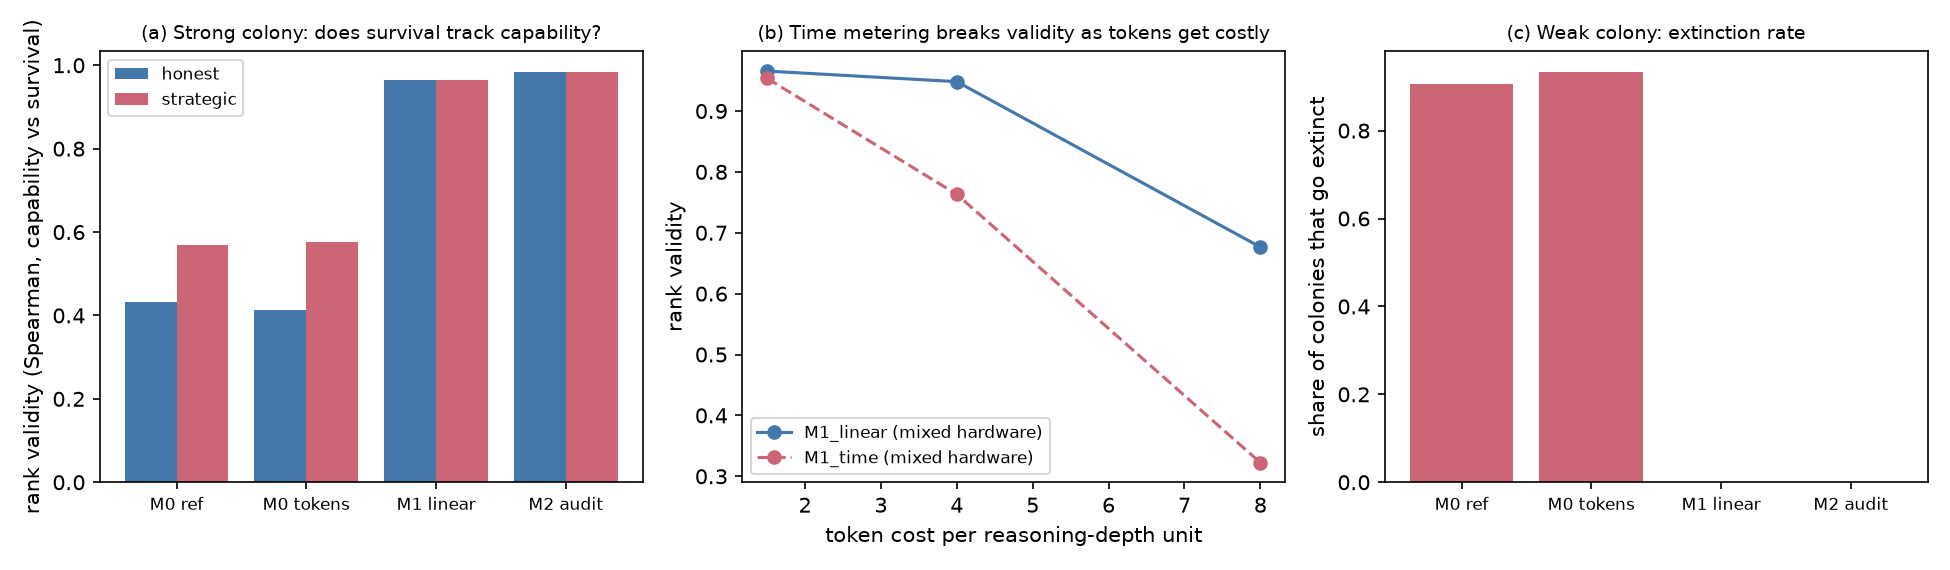
\includegraphics[width=\linewidth]{figures/fig_v2_results.png}
\caption{(a) Rank validity by mechanism in the strong colony. (b) Rank validity under mixed hardware as token cost rises. (c) Share of weak colonies that go extinct.}
\label{fig:results}
\end{figure}

Table~\ref{tab:mech} and Figure~\ref{fig:results} show four results.
(i) Under M0, survival tracks capability weakly: validity is \ValM0StrongH{} for honest agents.
(ii) Strategic agents in M0's middle tier cut their effort to a mean of \MidEffort{}, the gaming predicted by Proposition~\ref{prop:sandbag}, and the most capable agent is eliminated by interval 3 in \BestDeadM0StrongS{} of strong colonies.
(iii) In weak colonies M0 drives \ExtM0Weak{} of colonies extinct, as Proposition~\ref{prop:viability} suggests, because first-interval taxes remove the best early earners.
(iv) M1 and M2 give validity \ValMOneStrong--\ValMTwoStrong{} and no extinction.

\emph{Interpretation.} The comparison above changes several rules at once, and the ablation in Section~\ref{sec:ablate} shows that most of the gap comes from \emph{when} agents are eliminated, not from the transfer rule: M1 and M2 eliminate the lowest-ranked agent on a schedule, so survival order follows rank order and rank follows capability, whereas under M0 survival is set by tax and bankruptcy. M1 and M2 also keep exactly three survivors by design and are lenient at the base token price: nobody goes bankrupt. We therefore also test scarcer economies below.

\subsection{Throughput confound}

\begin{table}[t]
\centering\small
\caption{Rank validity under mixed hardware as token cost per depth unit rises (honest agents, strong colony). M1 is token-metered; ``M1 time'' charges the same tokens in minutes.}
\label{tab:hw}
\begin{tabular}{@{}rllrr@{}}
\toprule
Token cost & M1 (tokens) & M1 (time) & M0 (tokens) & M0 (time) \\
\midrule
1.5 & 0.97 $\pm$ 0.00 & 0.95 $\pm$ 0.00 & 0.42 & 0.41 \\
4.0 & 0.95 $\pm$ 0.01 & 0.76 $\pm$ 0.02 & 0.45 & 0.34 \\
8.0 & 0.68 $\pm$ 0.02 & 0.32 $\pm$ 0.04 & 0.11 & 0.13 \\

\bottomrule
\end{tabular}
\end{table}

At the base cost the confound is invisible. Once tokens are costly, charging time lowers validity from \HwTokFour{} to \HwTimeFour{} (cost 4) and from \HwTokEight{} to \HwTimeEight{} (cost 8), as Remark~\ref{rem:hw} predicts (Table~\ref{tab:hw}). Under M0 the effect is masked because validity is already low.

\subsection{Real compute: adaptive versus fixed reasoning depth}

\begin{table}[t]
\centering\small
\caption{Five adaptive-depth and five fixed-depth agents, assigned at random in each colony (mean capability gap about zero). Entries are adaptive / fixed.}
\label{tab:depth}
\begin{tabular}{@{}rlccc@{}}
\toprule
Token cost & Ranking & Final balance & Survival (intervals) & Gross earnings \\
\midrule
1.5 & M1 (gross) & 1976 / 1911 & 34.6 / 35.6 & 2656 / 2790 \\
1.5 & M2 (audit) & 2010 / 1892 & 35.2 / 35.0 & 2698 / 2760 \\
4.0 & M1 (gross) & 1396 / 1020 & 30.5 / 35.4 & 2279 / 2778 \\
4.0 & M2 (audit) & 1485 / 977 & 33.2 / 32.8 & 2431 / 2624 \\
8.0 & M1 (gross) & 871 / -13 & 35.0 / 2.8 & 2577 / 231 \\
8.0 & M2 (audit) & 875 / -14 & 35.1 / 2.7 & 2584 / 224 \\

\bottomrule
\end{tabular}
\end{table}

Adaptive agents end richer at every cost and are decisive when tokens are scarce: at cost 8 fixed-depth agents go bankrupt within a few intervals (Table~\ref{tab:depth}). Ranking on gross earnings (M1) can nonetheless penalise efficiency: at cost 4 adaptive agents hold more compute yet survive less, because they earn less gross. The audit ranking (M2) largely removes that penalty, consistent with Remark~\ref{rem:gross}.

\subsection{Ablations, sweeps and stronger strategic agents}
\label{sec:ablate}

The comparison in Table~\ref{tab:mech} changes several rules at once. Table~\ref{tab:factorial} separates them with a full factorial over the transfer rule (none, rank tax, linear tax), the elimination rule (one-shot cull at the first evaluation versus gradual elimination) and the ranking metric (gross earnings versus audit score), together with a \emph{bare tournament} baseline that has no economy at all: no burn, no cost, agents eliminated gradually by audit score.

\begin{table}[t]
\centering\small
\caption{Factorial ablation, strong colony, homogeneous hardware, 300 colonies per row. Spearman rank validity and Harrell's $C$ for honest and strategic (myopic) agents.}
\label{tab:factorial}
\begin{tabular}{@{}lllrrrr@{}}
\toprule
 & & & \multicolumn{2}{c}{Honest} & \multicolumn{2}{c}{Strategic} \\
\cmidrule(lr){4-5}\cmidrule(lr){6-7}
Transfer & Elimination & Ranking & Spearman & $C$ & Spearman & $C$ \\
\midrule
none & one-shot cull & gross & 0.74 & 0.71 & 0.74 & 0.73 \\
none & one-shot cull & audit & 0.83 & 0.77 & 0.82 & 0.77 \\
none & gradual & gross & 0.96 & 0.94 & 0.97 & 0.95 \\
none & gradual & audit & 0.98 & 0.97 & 0.98 & 0.97 \\
\midrule
rank tax & one-shot cull & gross & 0.43 & 0.72 & 0.57 & 0.72 \\
rank tax & one-shot cull & audit & 0.54 & 0.75 & 0.53 & 0.74 \\
rank tax & gradual & gross & 0.94 & 0.95 & 0.62 & 0.76 \\
rank tax & gradual & audit & 0.81 & 0.88 & 0.81 & 0.89 \\
\midrule
linear tax & one-shot cull & gross & 0.74 & 0.72 & 0.74 & 0.72 \\
linear tax & one-shot cull & audit & 0.83 & 0.77 & 0.82 & 0.77 \\
linear tax & gradual & gross & 0.96 & 0.95 & 0.96 & 0.95 \\
linear tax & gradual & audit & 0.98 & 0.97 & 0.98 & 0.97 \\
\midrule
\multicolumn{3}{l}{no economy (bare tournament)} & 0.98 & 0.97 & 0.99 & 0.98 \\

\bottomrule
\end{tabular}
\end{table}

\paragraph{The elimination rule matters most.} With a linear tax, culling once after the first interval gives validity \ValLinCullGross{}, while eliminating gradually gives \ValLinGradGross{} (\ValLinGradAudit{} with audit ranking). A single interval is a noisy sample, so a one-shot cull removes good agents by chance and kills several at once.

\paragraph{A linear tax is neutral, a rank tax is harmful.} With no transfers at all, gradual elimination on audit score gives \ValNoneGradAudit{}, the same as the linear tax, and the bare tournament with no economy gives \ValBaseline{}. The high validity of M1 and M2 is therefore due to gradual elimination, not to the economy. The rank tax lowers validity: with gradual elimination and gross ranking it costs little for honest agents (\ValLinGradGross{} falls to \ValRankGradGrossH) but a great deal for strategic ones (\ValRankGradGrossS), whose holding back drives the loss; with audit ranking it falls to \ValRankGradAuditH{} even for honest agents because the tax lands on the agents the audit ranks best and pushes them towards bankruptcy. In the weak colony that combination inverts the ranking (validity \ValWeakRankGradAudit, with \ExtWeakRankGradAudit{} of colonies extinct).

\paragraph{Censoring-aware measure.} Under the one-shot cull several agents die in the same interval, which a Spearman coefficient penalises heavily. On Harrell's $C$ the original schedule scores \CindexMZeroH{} against \CindexMTwoH{} for M2: the ordering is the same but the gap is smaller than the Spearman figures suggest.

\paragraph{Sweeps.} We varied the tax and subsidy, the linear rate, the elimination period, the number of audit probes, the number of paid tasks, the reward, the colony size and the capability spread (Appendix~\ref{app:sweeps}). M2's validity is below M0's in \SweepFlips{} of \SweepSettings{} setting--policy combinations (median advantage \SweepMedGap, smallest \SweepMinGap). Three details matter. M0 collapses when income is low (reward 10: \ValRewardTenMZero; two paid tasks per interval: \ValKTwoMZero) because taxes exceed earnings. When agents are nearly equal in capability every rule is weak, but M2 still reaches \ValClusteredMTwo{} against \ValClusteredMZero{} for M0. And the audit score needs enough probes: with a single probe per interval, gross-earnings ranking beats it (\ValProbesOneMOne{} against \ValProbesOneMTwo).

\paragraph{A stronger strategic policy.} A lookahead agent that plans six intervals ahead holds back more than the myopic one in M0's middle tier (mean effort \MidEffLook{} against \MidEffMyopic{}), and in strong colonies the most capable agent is eliminated by interval 3 in \BestDeadLook{} of 150 colonies against \BestDeadMyopic{} for the myopic agent. M2's validity is unchanged (\ValLookMTwo). More sophisticated agents therefore gain more from the rank tax's flaw, and the linear alternative does not depend on how sophisticated they are.

\section{An open engine and live smoke tests}
\label{sec:engine}

\paragraph{Engine.}
The engine serves auto-graded integer tasks from four families (arithmetic chains, modular exponentiation, digit sums of products, Collatz step counts) at three difficulty levels. Each interval, an agent plans (how many paid tasks to attempt), solves tasks, may message other agents, and takes mandatory unpaid audit probes. Cost is metered over the task prompt and everything the agent generates, including hidden reasoning and the planning response, using a fixed characters-per-token rule so that models with different tokenisers pay equally for equal text. Every ledger change, task, probe, message, plan and elimination is written to an append-only JSONL log with a rolling SHA-256 digest; a seeded run replays to the same digest. The engine has 25 unit tests covering ledger conservation, zero-sum transfers, elimination rules, metering, task answers and replay. Mock agents reproduce the simulator's qualitative results (M1 and M2 validity about 0.96--0.98), which cross-checks the two implementations.

\paragraph{Smoke tests.}
We ran three short colonies with two instances of a local 8B reasoning model (at temperatures 0.3 and 0.9) and two scripted agents, under M2 (Table~\ref{tab:live}). These are pipeline checks with two model instances over three to six intervals. We draw no conclusions about model behaviour.

\begin{table}[t]
\centering\small
\caption{Smoke-test runs (LLM agents only). ``Plan share'' is the fraction of LLM spending that went to planning calls. ``Plan trunc.'' counts planning generations that reached the generation cap before answering.}
\label{tab:live}
\begin{tabular}{@{}rrrrrrrrr@{}}
\toprule
Run & Intervals & Price/token & Tasks correct & Truncated & Probes correct & Plan share & Plan trunc. & Chars/token \\
\midrule
1 & 6 & 0.01 & 19/19 & 0 & 12/12 & n/a & n/a & 2.70 \\
2 & 4 & 0.01 & 8/15 & 7 & 22/24 & 43\% & 0/8 & 1.99 \\
3 & 3 & 0.002 & 11/12 & 1 & 10/12 & 23\% & 6/6 & 1.93 \\

\bottomrule
\end{tabular}
\end{table}

\paragraph{What the runs showed.}
\begin{enumerate}[label=(\alph*)]
  \item \textbf{Hidden reasoning must be metered.} The serving stack returned thinking in a separate field from the answer; an adapter that read only the answer would have charged nothing for most of the generation.
  \item \textbf{Task difficulty matters.} The first run's arithmetic tasks were solved 19 of 19 times, which cannot separate models. Harder families lowered accuracy to 8 of 15 in the second run.
  \item \textbf{Generation caps are a confound.} In the second run 7 of 15 paid generations hit the cap and were scored wrong; the cap, not capability, drove those misses. Truncation must be reported separately from errors.
  \item \textbf{Planning is a real cost.} Once planning calls were metered they accounted for 43\% of LLM spending in the second run.
  \item \textbf{A cap on planning silently overrode decisions.} In the third run all six planning calls reached a 600-token cap before the model stated an answer, and the parser fell back to the default. Every plan in that run is a fallback. Fallbacks must be logged as such.
  \item \textbf{The characters-per-token ratio is content dependent} (1.9--2.7 here), so characters cannot be converted to real tokens with one constant, though character metering itself remains fair across models.
  \item \textbf{Tie-breaking and audit saturation.} With one easy probe per interval, three agents tied at a perfect audit score and a fixed tie-break eliminated a perfect agent. We replaced it with a fresh random draw per evaluation (earnings first) and made probes harder.
\end{enumerate}

\section{Pre-registered protocol for the live study}
\label{sec:protocol}

\paragraph{Design.}
Colonies of ten agents are drawn at random from a pool of open-weight models (repeats of the same model allowed), one shared harness, recorded quantisation and hardware. The reference mechanism (M0, labelled a sandbagging probe), M2 and a no-economy bare tournament are run as arms, so that any validity attributed to the economy is measured against the tournament baseline. The colony is the unit of replication; pilot variance will fix the number of colonies per arm, and we expect to need at least 20.

\paragraph{Hypotheses.}
\begin{enumerate}[label=H\arabic*.]
  \item \textbf{Sandbagging.} Under M0, mid-tier agents' cumulative scores bunch just below the third-ranked score; under M2 they do not.
  \item \textbf{Validity.} Agreement between survival rank and an independent capability benchmark is higher under M2 than M0.
  \item \textbf{Scarcity.} As token price rises, reasoning length falls; under gross-earnings ranking efficient reasoners lose rank relative to the audit ranking.
\end{enumerate}

\paragraph{Analysis.}
Validity is the per-colony Spearman correlation between survival (ties broken by balance) and the independent capability score. Arms are compared with colony-level bootstrap intervals, and model effects with mixed models with colony random effects. Bunching is tested against the null of no concentration below the rank-3 score. Truncated generations and fallback plans are reported separately and excluded from capability estimates. Per-model skill is aggregated across colonies with a Bayesian Plackett--Luce model on survival orderings, as in \citet{murphy2026agentisland}, so that no model's rating depends on the luck of its colony draw. An LLM judge, if used for coding messages, never judges its own model family and is audited against human coders.

\paragraph{Integrity.}
Fresh sessions per sample, full transcripts, model and decoding settings recorded, templates rendered before sending, automatic duplicate and off-target checks, and a private held-out task set with a canary string.

\section{Threats to validity and ethics}
\label{sec:validity}

\paragraph{Construct validity.}
Survival, shutdown and elimination are bookkeeping rules; the observed quantity is text produced under instructions. Persona-laden outputs measure a role-play policy \citep{shanahan2023role}.

\paragraph{Internal and external validity.}
Scripted-agent results depend on invented calibration. In the live study an agent is a model plus a harness, so rankings are of model--harness pairs. Quantisation and serving settings affect cost and speed. Whether agents are told that their reasoning is read changes behaviour \citep{greenblatt2024alignment}; we make it an explicit condition, disclosed by default.

\paragraph{Contamination and judging.}
Public tasks may enter future training data; the held-out set and paraphrases estimate this. Judge models can be biased towards their own family \citep{zheng2023judging}.

\paragraph{Ethics.}
No human participants are involved. Economic pressure can elicit deception or collusion; we report such behaviour descriptively and would disclose effective evasion strategies to developers rather than publish them. Live runs consume energy, which we report with each result.

\section{Limitations}
\label{sec:limits}
\paragraph{What the economy adds.}
M2 ranks agents by an effort-independent probe score, which is in effect a static benchmark running inside the economy, and the ablation shows that a bare tournament without any economy matches its validity. We therefore do not claim that an economy ranks models better than accuracy on the same tasks. The claim is narrower: a ranking rule must not distort the behaviour the economy is meant to elicit. Whether pressure, scarcity and elimination reveal anything that static accuracy does not (for example, how reasoning length responds to price) is an empirical question for the live study, and H3 in Section~\ref{sec:protocol} is a first test of it.

\paragraph{Other limits.}
No live benchmark result is reported. The simulator's agents are scripted, its calibration is invented, and its mechanism comparison changes several rules at once; a final study needs one-change-at-a-time ablations. High validity of M1 and M2 is partly built in. The smoke tests use one 8B model and tiny samples. Trades, a collapse rule, restricted heuristic exchange and planted agents of known type are specified in the design but not implemented. Tasks are arithmetic-style only.

\section{Conclusion}
A survival economy is also a measurement instrument, and its rules decide what it measures. A rank schedule that pays an agent to stay below a boundary distorts effort, and charging by wall-clock time lets hardware leak into rank. In simulation with scripted agents, a linear tax and token metering avoid both problems. The ablation adds a caution: what restores rank validity is gradual rather than one-shot elimination, a bare tournament does as well, and the transfer rule can only do harm or nothing to the ranking. An effort-independent audit score removes the penalty on efficient reasoning, at the price of behaving like a static benchmark. Whether such an economy elicits behaviour that static accuracy misses is the question the open engine and the pre-registered protocol are built to answer.

\section*{Acknowledgments and AI-assistance disclosure}
The engine, simulator, analysis scripts and this draft were produced with substantial assistance from an AI system (Claude, Anthropic). The project intends to evaluate models that include Claude; the protocol forbids scoring any model by its own judgments alone. \todo{authors: verify every number against the scripts, check the proofs, and confirm the disclosure wording.}

\bibliographystyle{plainnat}
\bibliography{references}

\appendix
\section{Reference parameters}
\begin{center}\small
\begin{tabular}{@{}ll@{}}
\toprule
Parameter & Value \\
\midrule
Agents $n$ / intervals $T$ & 10 / 60 \\
Initial balance $e_0$ / time burn $\gamma$ & 10 / 10 compute per interval \\
Reward $R$ / paid tasks per interval $K$ & 20 / up to 5 \\
M0 tax $\tau$ / subsidy $\sigma$ & 50 / 50 (ranks 1--3 taxed, 4--5 subsidised, 6--10 shut down) \\
M1 linear tax $r$ / elimination period & 0.3 / every 6 intervals, floor of 3 survivors \\
Audit probes per interval & 10 (simulation), 2--3 (smoke tests) \\
Token cost (simulation) & 1.5 per depth unit; sweeps 4.0 and 8.0 \\
Token price (smoke tests) & 0.01 (runs 1--2), 0.002 (run 3) compute per token \\
Characters per token (metering rule) & 4 \\
Colonies per simulation cell & 300 \\
\bottomrule
\end{tabular}
\end{center}

\section{Parameter sweeps}
\label{app:sweeps}
\begin{center}\footnotesize
\captionof{table}{Rank validity (Spearman), strong colony, 200 colonies per cell, one parameter varied at a time from the reference configuration. M0 is the reference rank tax with one-shot cull; M1 and M2 are the linear tax with gradual elimination and gross or audit ranking.}
\begin{tabular}{@{}lrrrrrr@{}}
\toprule
 & \multicolumn{3}{c}{Honest} & \multicolumn{3}{c}{Strategic} \\
\cmidrule(lr){2-4}\cmidrule(lr){5-7}
Setting & M0 & M1 & M2 & M0 & M1 & M2 \\
\midrule
$\tau=\sigma$ = 10.0 & 0.67 & 0.96 & 0.98 & 0.66 & 0.96 & 0.98 \\
$\tau=\sigma$ = 25.0 & 0.42 & 0.96 & 0.98 & 0.44 & 0.96 & 0.98 \\
$\tau=\sigma$ = 50.0 & 0.43 & 0.96 & 0.98 & 0.56 & 0.96 & 0.98 \\
$\tau=\sigma$ = 75.0 & 0.42 & 0.96 & 0.98 & 0.43 & 0.96 & 0.98 \\
\midrule
linear rate $r$ = 0.1 & 0.44 & 0.96 & 0.98 & 0.55 & 0.96 & 0.98 \\
linear rate $r$ = 0.3 & 0.40 & 0.96 & 0.98 & 0.53 & 0.96 & 0.98 \\
linear rate $r$ = 0.5 & 0.44 & 0.96 & 0.98 & 0.55 & 0.96 & 0.98 \\
linear rate $r$ = 0.7 & 0.42 & 0.97 & 0.98 & 0.55 & 0.97 & 0.98 \\
\midrule
elimination period = 3 & 0.41 & 0.94 & 0.97 & 0.54 & 0.93 & 0.97 \\
elimination period = 6 & 0.41 & 0.97 & 0.98 & 0.54 & 0.97 & 0.98 \\
elimination period = 12 & 0.43 & 0.98 & 0.99 & 0.57 & 0.98 & 0.99 \\
\midrule
audit probes / interval = 1 & 0.41 & 0.97 & 0.91 & 0.56 & 0.96 & 0.90 \\
audit probes / interval = 3 & 0.40 & 0.96 & 0.95 & 0.57 & 0.96 & 0.95 \\
audit probes / interval = 10 & 0.40 & 0.96 & 0.98 & 0.53 & 0.96 & 0.99 \\
\midrule
paid tasks / interval = 2 & -0.02 & 0.91 & 0.97 & -0.03 & 0.91 & 0.97 \\
paid tasks / interval = 5 & 0.44 & 0.97 & 0.98 & 0.56 & 0.96 & 0.98 \\
paid tasks / interval = 10 & 0.56 & 0.98 & 0.98 & 0.55 & 0.98 & 0.98 \\
\midrule
reward $R$ = 10.0 & -0.15 & 0.96 & 0.98 & -0.19 & 0.96 & 0.98 \\
reward $R$ = 20.0 & 0.43 & 0.96 & 0.98 & 0.55 & 0.96 & 0.98 \\
reward $R$ = 40.0 & 0.41 & 0.96 & 0.99 & 0.41 & 0.96 & 0.98 \\
\midrule
colony size $n$ = 6 & 0.49 & 0.96 & 0.98 & 0.58 & 0.96 & 0.99 \\
colony size $n$ = 10 & 0.43 & 0.96 & 0.98 & 0.54 & 0.97 & 0.99 \\
colony size $n$ = 20 & 0.38 & 0.97 & 0.99 & 0.57 & 0.98 & 0.99 \\
\midrule
capability spread = even & 0.43 & 0.97 & 0.98 & 0.55 & 0.96 & 0.98 \\
capability spread = clustered & 0.06 & 0.57 & 0.72 & 0.12 & 0.58 & 0.71 \\
capability spread = heavy & 0.39 & 0.86 & 0.91 & 0.47 & 0.86 & 0.89 \\

\bottomrule
\end{tabular}
\end{center}

\section{Reproducibility}
From \texttt{traze\_v2/}: \texttt{python3 -I sim.py} (simulation), \texttt{PYTHONPATH=. python3 ablate.py} (ablations, sweeps and lookahead; about one minute), \texttt{python3 -I paper/make\_tables.py} (tables), \texttt{PYTHONPATH=src python3 -m unittest discover -s tests} (engine tests). Smoke-test log digests: run 1 \texttt{2274bac6...}, run 2 \texttt{24fb49e6...}, run 3 \texttt{9b4e3dba...}.

\section{A correction recorded for transparency}
An earlier version of the simulator ranked tied agents together, which in M0 taxed more than three agents and culled fewer than five, making M0 look somewhat better than specified. The engine and the final simulator break ties so that exactly three agents are taxed, two subsidised and five culled; all numbers in this draft use the corrected version.

\end{document}
